\documentclass{standalone}
\usepackage{tikz}
\usetikzlibrary{patterns, positioning}


\begin{document}
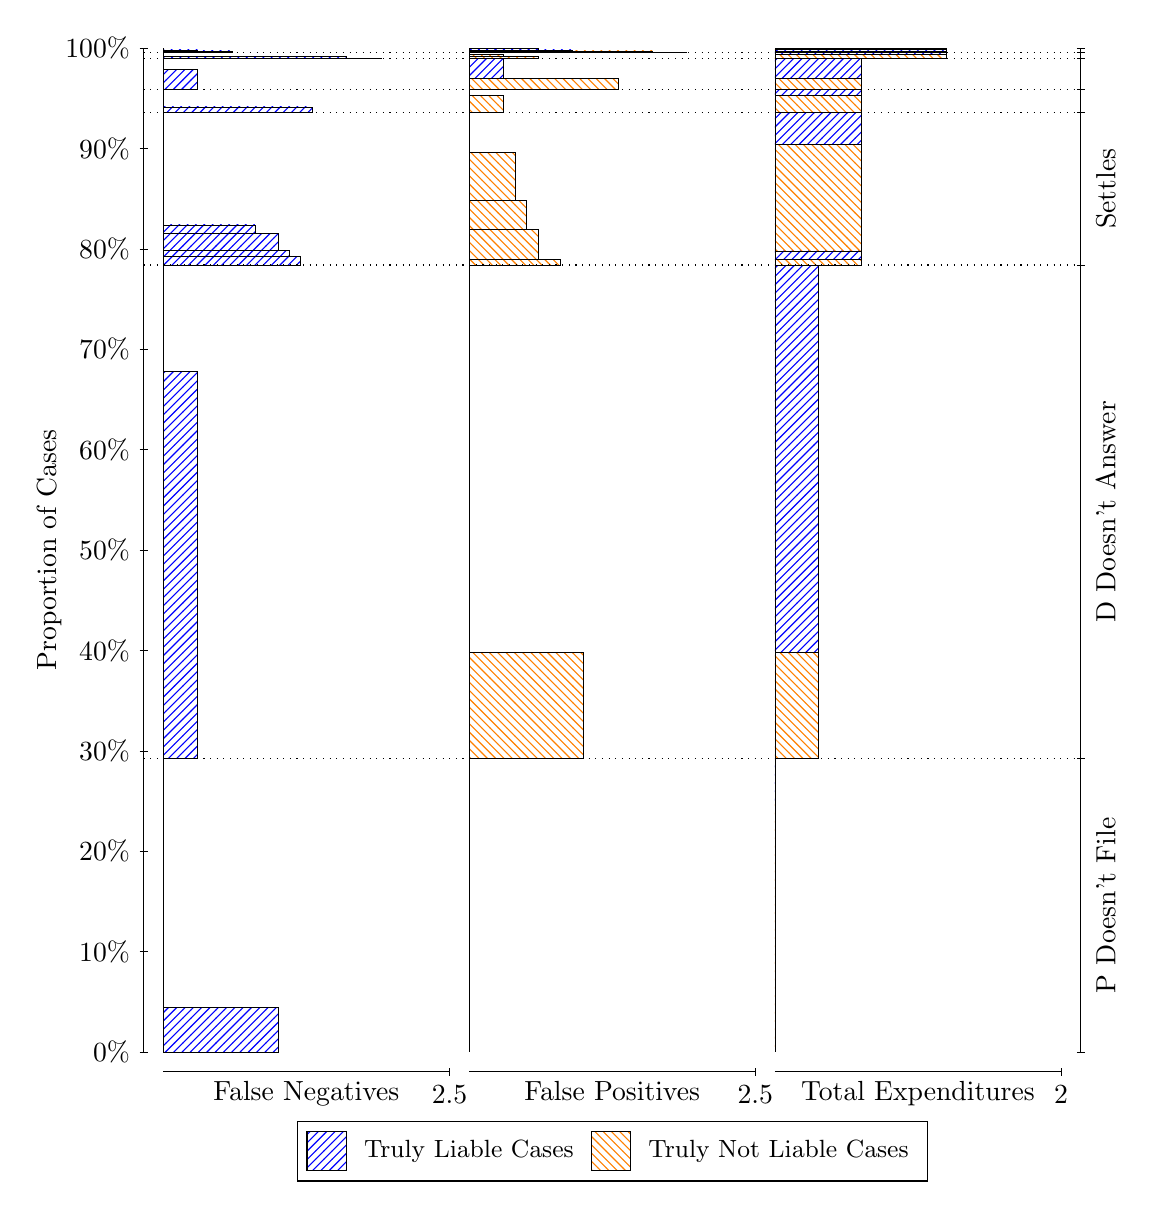
\begin{tikzpicture}
\draw[black, very thin] (1.5,1.75) -- (1.5,14.5);
\node[rotate=90, text=black, anchor=center] at (0.3, 8.125) {Proportion of Cases};
\draw[black, very thin] (1.45,1.75) -- (1.55,1.75);
\node[text=black, anchor=east] at (1.45, 1.75) {0\%};
\draw[black, very thin] (1.45,3.025) -- (1.55,3.025);
\node[text=black, anchor=east] at (1.45, 3.025) {10\%};
\draw[black, very thin] (1.45,4.3) -- (1.55,4.3);
\node[text=black, anchor=east] at (1.45, 4.3) {20\%};
\draw[black, very thin] (1.45,5.575) -- (1.55,5.575);
\node[text=black, anchor=east] at (1.45, 5.575) {30\%};
\draw[black, very thin] (1.45,6.85) -- (1.55,6.85);
\node[text=black, anchor=east] at (1.45, 6.85) {40\%};
\draw[black, very thin] (1.45,8.125) -- (1.55,8.125);
\node[text=black, anchor=east] at (1.45, 8.125) {50\%};
\draw[black, very thin] (1.45,9.4) -- (1.55,9.4);
\node[text=black, anchor=east] at (1.45, 9.4) {60\%};
\draw[black, very thin] (1.45,10.675) -- (1.55,10.675);
\node[text=black, anchor=east] at (1.45, 10.675) {70\%};
\draw[black, very thin] (1.45,11.95) -- (1.55,11.95);
\node[text=black, anchor=east] at (1.45, 11.95) {80\%};
\draw[black, very thin] (1.45,13.225) -- (1.55,13.225);
\node[text=black, anchor=east] at (1.45, 13.225) {90\%};
\draw[black, very thin] (1.45,14.5) -- (1.55,14.5);
\node[text=black, anchor=east] at (1.45, 14.5) {100\%};

\draw[black, very thin] (13.4,1.75) -- (13.4,14.5);
\draw[black, very thin] (13.35,1.75) -- (13.45,1.75);
\node[anchor=west] at (13.35, 1.75) {};
\draw[black, very thin] (13.35,5.4764) -- (13.45,5.4764);
\node[anchor=west] at (13.35, 5.4764) {};
\draw[black, very thin] (13.35,11.744) -- (13.45,11.744);
\node[anchor=west] at (13.35, 11.744) {};
\draw[black, very thin] (13.35,13.682) -- (13.45,13.682);
\node[anchor=west] at (13.35, 13.682) {};
\draw[black, very thin] (13.35,13.972) -- (13.45,13.972);
\node[anchor=west] at (13.35, 13.972) {};
\draw[black, very thin] (13.35,14.366) -- (13.45,14.366);
\node[anchor=west] at (13.35, 14.366) {};
\draw[black, very thin] (13.35,14.441) -- (13.45,14.441);
\node[anchor=west] at (13.35, 14.441) {};
\draw[black, very thin] (13.35,14.5) -- (13.45,14.5);
\node[anchor=west] at (13.35, 14.5) {};

\draw[black, very thin, pattern color=blue, pattern=north east lines] (1.75,1.75) rectangle (3.2033,2.312);
\draw[black, very thin, pattern color=orange, pattern=north west lines] (1.75,2.312) rectangle (1.75,5.4764);
\draw[black, very thin, pattern color=blue, pattern=north east lines] (1.75,5.4764) rectangle (2.186,10.394);
\draw[black, very thin, pattern color=orange, pattern=north west lines] (1.75,10.394) rectangle (1.75,11.744);
\draw[black, very thin, pattern color=blue, pattern=north east lines] (1.75,11.744) rectangle (3.494,11.855);
\draw[black, very thin, pattern color=blue, pattern=north east lines] (1.75,11.855) rectangle (3.3487,11.933);
\draw[black, very thin, pattern color=blue, pattern=north east lines] (1.75,11.933) rectangle (3.2033,12.149);
\draw[black, very thin, pattern color=blue, pattern=north east lines] (1.75,12.149) rectangle (2.9127,12.255);
\draw[black, very thin, pattern color=orange, pattern=north west lines] (1.75,12.255) rectangle (1.75,13.682);
\draw[black, very thin, pattern color=blue, pattern=north east lines] (1.75,13.682) rectangle (3.6393,13.753);
\draw[black, very thin, pattern color=orange, pattern=north west lines] (1.75,13.753) rectangle (1.75,13.972);
\draw[black, very thin, pattern color=blue, pattern=north east lines] (1.75,13.972) rectangle (2.186,14.226);
\draw[black, very thin, pattern color=orange, pattern=north west lines] (1.75,14.226) rectangle (1.75,14.366);
\draw[black, very thin, pattern color=blue, pattern=north east lines] (1.75,14.366) rectangle (4.5113,14.372);
\draw[black, very thin, pattern color=blue, pattern=north east lines] (1.75,14.372) rectangle (4.0753,14.389);
\draw[black, very thin, pattern color=orange, pattern=north west lines] (1.75,14.389) rectangle (1.75,14.441);
\draw[black, very thin, pattern color=blue, pattern=north east lines] (1.75,14.441) rectangle (2.622,14.464);
\draw[black, very thin, pattern color=blue, pattern=north east lines] (1.75,14.464) rectangle (2.186,14.477);
\draw[black, very thin, pattern color=orange, pattern=north west lines] (1.75,14.477) rectangle (1.75,14.5);
\draw[black, very thin, pattern color=orange, pattern=north west lines] (5.6333,1.75) rectangle (5.6333,4.9144);
\draw[black, very thin, pattern color=blue, pattern=north east lines] (5.6333,4.9144) rectangle (5.6333,5.4764);
\draw[black, very thin, pattern color=orange, pattern=north west lines] (5.6333,5.4764) rectangle (7.0867,6.8264);
\draw[black, very thin, pattern color=blue, pattern=north east lines] (5.6333,6.8264) rectangle (5.6333,11.744);
\draw[black, very thin, pattern color=orange, pattern=north west lines] (5.6333,11.744) rectangle (6.796,11.818);
\draw[black, very thin, pattern color=orange, pattern=north west lines] (5.6333,11.818) rectangle (6.5053,12.193);
\draw[black, very thin, pattern color=orange, pattern=north west lines] (5.6333,12.193) rectangle (6.36,12.564);
\draw[black, very thin, pattern color=orange, pattern=north west lines] (5.6333,12.564) rectangle (6.2147,13.171);
\draw[black, very thin, pattern color=blue, pattern=north east lines] (5.6333,13.171) rectangle (5.6333,13.682);
\draw[black, very thin, pattern color=orange, pattern=north west lines] (5.6333,13.682) rectangle (6.0693,13.901);
\draw[black, very thin, pattern color=blue, pattern=north east lines] (5.6333,13.901) rectangle (5.6333,13.972);
\draw[black, very thin, pattern color=orange, pattern=north west lines] (5.6333,13.972) rectangle (7.5227,14.112);
\draw[black, very thin, pattern color=blue, pattern=north east lines] (5.6333,14.112) rectangle (6.0693,14.366);
\draw[black, very thin, pattern color=orange, pattern=north west lines] (5.6333,14.366) rectangle (6.5053,14.396);
\draw[black, very thin, pattern color=orange, pattern=north west lines] (5.6333,14.396) rectangle (6.0693,14.418);
\draw[black, very thin, pattern color=blue, pattern=north east lines] (5.6333,14.418) rectangle (5.6333,14.441);
\draw[black, very thin, pattern color=orange, pattern=north west lines] (5.6333,14.441) rectangle (8.3947,14.445);
\draw[black, very thin, pattern color=orange, pattern=north west lines] (5.6333,14.445) rectangle (7.9587,14.463);
\draw[black, very thin, pattern color=blue, pattern=north east lines] (5.6333,14.463) rectangle (6.9413,14.477);
\draw[black, very thin, pattern color=blue, pattern=north east lines] (5.6333,14.477) rectangle (6.5053,14.5);
\draw[black, very thin, pattern color=orange, pattern=north west lines] (9.5167,1.75) rectangle (9.5167,4.9144);
\draw[black, very thin, pattern color=blue, pattern=north east lines] (9.5167,4.9144) rectangle (9.5167,5.4764);
\draw[black, very thin, pattern color=orange, pattern=north west lines] (9.5167,5.4764) rectangle (10.062,6.8264);
\draw[black, very thin, pattern color=blue, pattern=north east lines] (9.5167,6.8264) rectangle (10.062,11.744);
\draw[black, very thin, pattern color=orange, pattern=north west lines] (9.5167,11.744) rectangle (10.607,11.818);
\draw[black, very thin, pattern color=blue, pattern=north east lines] (9.5167,11.818) rectangle (10.607,11.924);
\draw[black, very thin, pattern color=orange, pattern=north west lines] (9.5167,11.924) rectangle (10.607,13.277);
\draw[black, very thin, pattern color=blue, pattern=north east lines] (9.5167,13.277) rectangle (10.607,13.682);
\draw[black, very thin, pattern color=orange, pattern=north west lines] (9.5167,13.682) rectangle (10.607,13.901);
\draw[black, very thin, pattern color=blue, pattern=north east lines] (9.5167,13.901) rectangle (10.607,13.972);
\draw[black, very thin, pattern color=orange, pattern=north west lines] (9.5167,13.972) rectangle (10.607,14.112);
\draw[black, very thin, pattern color=blue, pattern=north east lines] (9.5167,14.112) rectangle (10.607,14.366);
\draw[black, very thin, pattern color=orange, pattern=north west lines] (9.5167,14.366) rectangle (11.697,14.418);
\draw[black, very thin, pattern color=blue, pattern=north east lines] (9.5167,14.418) rectangle (11.697,14.441);
\draw[black, very thin, pattern color=orange, pattern=north west lines] (9.5167,14.441) rectangle (11.697,14.459);
\draw[black, very thin, pattern color=blue, pattern=north east lines] (9.5167,14.459) rectangle (11.697,14.482);
\draw[black, very thin, pattern color=orange, pattern=north west lines] (9.5167,14.482) rectangle (11.697,14.486);
\draw[black, very thin, pattern color=blue, pattern=north east lines] (9.5167,14.486) rectangle (11.697,14.5);
\draw[black, dotted] (1.5,5.4764) -- (13.4,5.4764);
\draw[black, dotted] (1.5,11.744) -- (13.4,11.744);
\draw[black, dotted] (1.5,13.682) -- (13.4,13.682);
\draw[black, dotted] (1.5,13.972) -- (13.4,13.972);
\draw[black, dotted] (1.5,14.366) -- (13.4,14.366);
\draw[black, dotted] (1.5,14.441) -- (13.4,14.441);
\draw[black, very thin] (1.75,1.5) -- (5.3833,1.5);
\node[text=black, anchor=north] at (3.5667, 1.5) {False Negatives};
\draw[black, very thin] (5.3833,1.45) -- (5.3833,1.55);
\node[text=black, anchor=north] at (5.3833, 1.45) {2.5};

\draw[black, very thin] (5.6333,1.5) -- (9.2667,1.5);
\node[text=black, anchor=north] at (7.45, 1.5) {False Positives};
\draw[black, very thin] (9.2667,1.45) -- (9.2667,1.55);
\node[text=black, anchor=north] at (9.2667, 1.45) {2.5};

\draw[black, very thin] (9.5167,1.5) -- (13.15,1.5);
\node[text=black, anchor=north] at (11.333, 1.5) {Total Expenditures};
\draw[black, very thin] (13.15,1.45) -- (13.15,1.55);
\node[text=black, anchor=north] at (13.15, 1.45) {2};

\node[text=black, centered, rotate=90] at (13.72, 3.6132) {P Doesn't File};
\node[text=black, centered, rotate=90] at (13.72, 8.6102) {D Doesn't Answer};
\node[text=black, centered, rotate=90] at (13.72, 12.713) {Settles};





\draw (7.449999999999999,1.5) node[draw=none] (baseCoordinate) {};
\begin{scope}[align=center]
        \matrix[scale=0.5, draw=black, below=0.5cm of baseCoordinate, nodes={draw}, column sep=0.1cm]{
            \node[rectangle, draw, minimum width=0.5cm, minimum height=0.5cm, pattern color=blue, pattern=north east lines] {}; &
            \node[draw=none, font=\small, text=black] (B) {Truly Liable Cases}; &
            \node[rectangle, draw, minimum width=0.5cm, minimum height=0.5cm, pattern color=orange, pattern=north west lines] {}; &
            \node[draw=none, font=\small, text=black] (B) {Truly Not Liable Cases}; \\
            };
\end{scope}

\end{tikzpicture}
\end{document}